% This file was created with tikzplotlib v0.9.16.
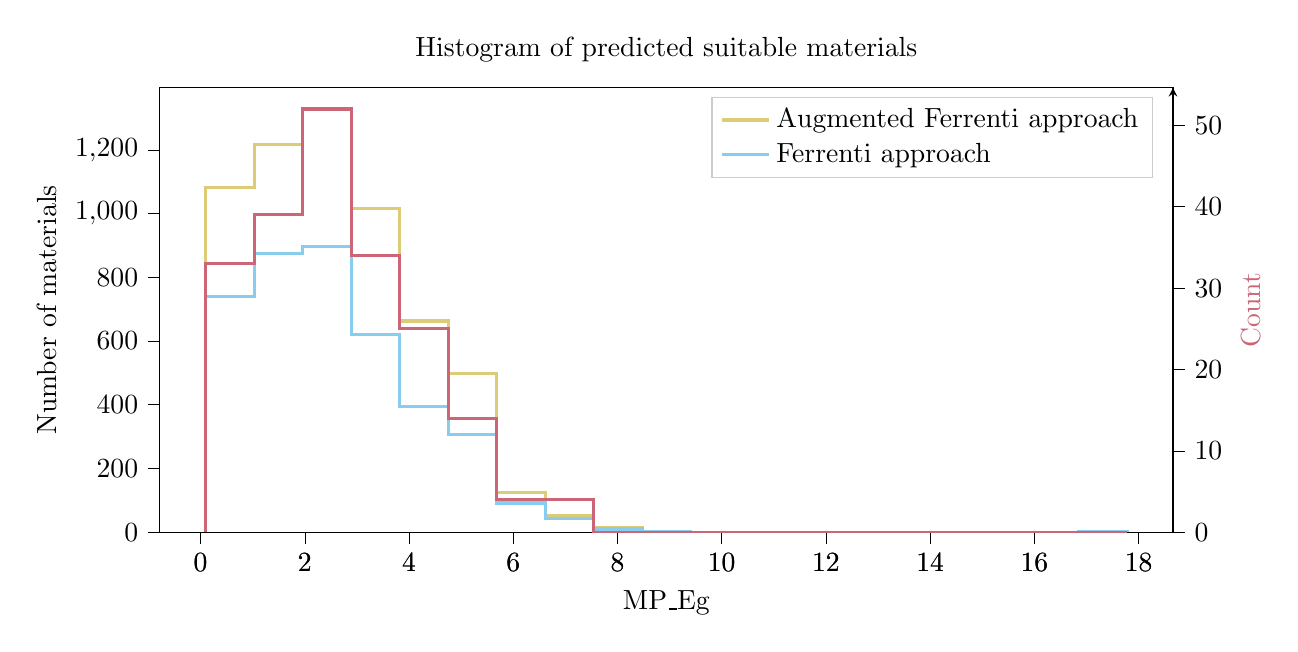
\begin{tikzpicture}

\definecolor{color0}{rgb}{0.866666666666667,0.8,0.466666666666667}
\definecolor{color1}{rgb}{0.533333333333333,0.8,0.933333333333333}
\definecolor{color2}{rgb}{0.8,0.4,0.466666666666667}

\begin{axis}[
height=2.8444876158848764in,
legend cell align={left},
legend style={fill opacity=0.8, draw opacity=1, text opacity=1, draw=white!80!black},
tick align=outside,
tick pos=left,
title={Histogram of predicted suitable materials},
width=5.688975231769753in,
x grid style={white!69.0196078431373!black},
xlabel={MP\_Eg},
xmin=-0.78335, xmax=18.65915,
xtick style={color=black},
y grid style={white!69.0196078431373!black},
ylabel={Number of materials},
ymin=0, ymax=1394.4,
ytick style={color=black}
]
\path [draw=color0, very thick]
(axis cs:0.1004,0)
--(axis cs:0.1004,1081)
--(axis cs:1.03066315789474,1081)
--(axis cs:1.03066315789474,1217)
--(axis cs:1.96092631578947,1217)
--(axis cs:1.96092631578947,1328)
--(axis cs:2.89118947368421,1328)
--(axis cs:2.89118947368421,1015)
--(axis cs:3.82145263157895,1015)
--(axis cs:3.82145263157895,663)
--(axis cs:4.75171578947368,663)
--(axis cs:4.75171578947368,498)
--(axis cs:5.68197894736842,498)
--(axis cs:5.68197894736842,125)
--(axis cs:6.61224210526316,125)
--(axis cs:6.61224210526316,53)
--(axis cs:7.54250526315789,53)
--(axis cs:7.54250526315789,13)
--(axis cs:8.47276842105263,13)
--(axis cs:8.47276842105263,1)
--(axis cs:9.40303157894737,1)
--(axis cs:9.40303157894737,0)
--(axis cs:10.3332947368421,0)
--(axis cs:10.3332947368421,0)
--(axis cs:11.2635578947368,0)
--(axis cs:11.2635578947368,0)
--(axis cs:12.1938210526316,0)
--(axis cs:12.1938210526316,0)
--(axis cs:13.1240842105263,0)
--(axis cs:13.1240842105263,0)
--(axis cs:14.0543473684211,0)
--(axis cs:14.0543473684211,0)
--(axis cs:14.9846105263158,0)
--(axis cs:14.9846105263158,0)
--(axis cs:15.9148736842105,0)
--(axis cs:15.9148736842105,0)
--(axis cs:16.8451368421053,0)
--(axis cs:16.8451368421053,1)
--(axis cs:17.7754,1)
--(axis cs:17.7754,0);
\addlegendimage{line legend, draw=color0, very thick}
\addlegendentry{Augmented Ferrenti approach}

\path [draw=color1, very thick]
(axis cs:0.1004,0)
--(axis cs:0.1004,740)
--(axis cs:1.03066315789474,740)
--(axis cs:1.03066315789474,875)
--(axis cs:1.96092631578947,875)
--(axis cs:1.96092631578947,897)
--(axis cs:2.89118947368421,897)
--(axis cs:2.89118947368421,621)
--(axis cs:3.82145263157895,621)
--(axis cs:3.82145263157895,394)
--(axis cs:4.75171578947368,394)
--(axis cs:4.75171578947368,307)
--(axis cs:5.68197894736842,307)
--(axis cs:5.68197894736842,92)
--(axis cs:6.61224210526316,92)
--(axis cs:6.61224210526316,43)
--(axis cs:7.54250526315789,43)
--(axis cs:7.54250526315789,10)
--(axis cs:8.47276842105263,10)
--(axis cs:8.47276842105263,1)
--(axis cs:9.40303157894737,1)
--(axis cs:9.40303157894737,0)
--(axis cs:10.3332947368421,0)
--(axis cs:10.3332947368421,0)
--(axis cs:11.2635578947368,0)
--(axis cs:11.2635578947368,0)
--(axis cs:12.1938210526316,0)
--(axis cs:12.1938210526316,0)
--(axis cs:13.1240842105263,0)
--(axis cs:13.1240842105263,0)
--(axis cs:14.0543473684211,0)
--(axis cs:14.0543473684211,0)
--(axis cs:14.9846105263158,0)
--(axis cs:14.9846105263158,0)
--(axis cs:15.9148736842105,0)
--(axis cs:15.9148736842105,0)
--(axis cs:16.8451368421053,0)
--(axis cs:16.8451368421053,1)
--(axis cs:17.7754,1)
--(axis cs:17.7754,0);
\addlegendimage{line legend, draw=color1, very thick}
\addlegendentry{Ferrenti approach}

\end{axis}

\begin{axis}[
axis y line=right,
height=2.8444876158848764in,
tick align=outside,
width=5.688975231769753in,
x grid style={white!69.0196078431373!black},
xmin=-0.78335, xmax=18.65915,
xtick pos=left,
xtick style={color=black},
y grid style={white!69.0196078431373!black},
ylabel=\textcolor{color2}{Count},
ymin=0, ymax=54.6,
ytick pos=right,
ytick style={color=black},
yticklabel style={anchor=west}
]
\path [draw=color2, very thick]
(axis cs:0.1004,0)
--(axis cs:0.1004,33)
--(axis cs:1.03066315789474,33)
--(axis cs:1.03066315789474,39)
--(axis cs:1.96092631578947,39)
--(axis cs:1.96092631578947,52)
--(axis cs:2.89118947368421,52)
--(axis cs:2.89118947368421,34)
--(axis cs:3.82145263157895,34)
--(axis cs:3.82145263157895,25)
--(axis cs:4.75171578947368,25)
--(axis cs:4.75171578947368,14)
--(axis cs:5.68197894736842,14)
--(axis cs:5.68197894736842,4)
--(axis cs:6.61224210526316,4)
--(axis cs:6.61224210526316,4)
--(axis cs:7.54250526315789,4)
--(axis cs:7.54250526315789,0)
--(axis cs:8.47276842105263,0)
--(axis cs:8.47276842105263,0)
--(axis cs:9.40303157894737,0)
--(axis cs:9.40303157894737,0)
--(axis cs:10.3332947368421,0)
--(axis cs:10.3332947368421,0)
--(axis cs:11.2635578947368,0)
--(axis cs:11.2635578947368,0)
--(axis cs:12.1938210526316,0)
--(axis cs:12.1938210526316,0)
--(axis cs:13.1240842105263,0)
--(axis cs:13.1240842105263,0)
--(axis cs:14.0543473684211,0)
--(axis cs:14.0543473684211,0)
--(axis cs:14.9846105263158,0)
--(axis cs:14.9846105263158,0)
--(axis cs:15.9148736842105,0)
--(axis cs:15.9148736842105,0)
--(axis cs:16.8451368421053,0)
--(axis cs:16.8451368421053,0)
--(axis cs:17.7754,0)
--(axis cs:17.7754,0);
\end{axis}

\end{tikzpicture}
